%\title{Modelo de Projeto de pesquisa}
%% abtex2-modelo-projeto-pesquisa.tex, v-1.9 laurocesar
%% Copyright 2012-2013 by abnTeX2 group at http://abntex2.googlecode.com/ 
%%
%% This work may be distributed and/or modified under the
%% conditions of the LaTeX Project Public License, either version 1.3
%% of this license or (at your option) any later version.
%% The latest version of this license is in
%%   http://www.latex-project.org/lppl.txt
%% and version 1.3 or later is part of all distributions of LaTeX
%% version 2005/12/01 or later.
%%
%% This work has the LPPL maintenance status `maintained'.
%% 
%% The Current Maintainer of this work is the abnTeX2 team, led
%% by Lauro César Araujo. Further information are available on 
%% http://abntex2.googlecode.com/
%%
%% This work consists of the files abntex2-modelo-projeto-pesquisa.tex
%% and abntex2-modelo-references.bib
%%

% ------------------------------------------------------------------------
% ------------------------------------------------------------------------
% abnTeX2: Modelo de Projeto de pesquisa em conformidade com 
% ABNT NBR 15287:2011 Informação e documentação - Projeto de pesquisa -
% Apresentação 
% ------------------------------------------------------------------------ 
% ------------------------------------------------------------------------

\documentclass[
	% -- opções da classe memoir --
	12pt,				% tamanho da fonte
	openright,			% capítulos começam em pág ímpar (insere página vazia caso preciso)
	oneside,			% para impressão em verso e anverso. Oposto a oneside
	a4paper,			% tamanho do papel. 
	% -- opções da classe abntex2 --
	%chapter=TITLE,		% títulos de capítulos convertidos em letras maiúsculas
	%section=TITLE,		% títulos de seções convertidos em letras maiúsculas
	%subsection=TITLE,	% títulos de subseções convertidos em letras maiúsculas
	%subsubsection=TITLE,% títulos de subsubseções convertidos em letras maiúsculas
	% -- opções do pacote babel --
	english,			% idioma adicional para hifenização
	%french,				% idioma adicional para hifenização
	%spanish,			% idioma adicional para hifenização
	brazil,				% o último idioma é o principal do documento
	]{abntex2}

% ---
% PACOTES
% ---

% ---
% Pacotes fundamentais 
% ---
\usepackage{lmodern}			% Usa a fonte Latin Modern
\usepackage[T1]{fontenc}		% Selecao de codigos de fonte.
\usepackage[utf8]{inputenc}		% Codificacao do documento (conversão automática dos acentos)
\usepackage{indentfirst}		% Indenta o primeiro parágrafo de cada seção.
\usepackage{color}				% Controle das cores
\usepackage{graphicx}			% Inclusão de gráficos
\graphicspath{ {./} }
\usepackage{microtype} 			% para melhorias de justificação
\usepackage{multirow}			% para tabelas com celulas mergeadas
\usepackage{array}			% para multilinhas nas celulas

% ---

\newcolumntype{L}{>{\centering\arraybackslash}m{1cm}}
\newcolumntype{M}{>{\centering\arraybackslash}m{3cm}}

\newcommand{\marcos}[1]{{\color{blue}{MARCOS: #1}}}

% ---
% Pacotes adicionais, usados apenas no âmbito do Modelo Canônico do abnteX2
% ---
\usepackage{lipsum}				% para geração de dummy text
% ---

% ---
% Pacotes de citações
% ---
\usepackage[brazilian,hyperpageref]{backref}	 % Paginas com as citações na bibl
\usepackage[alf]{abntex2cite}	% Citações padrão ABNT

% --- 
% CONFIGURAÇÕES DE PACOTES
% --- 

% ---
% Configurações do pacote backref
% Usado sem a opção hyperpageref de backref
\renewcommand{\backrefpagesname}{Citado na(s) página(s):~}
% Texto padrão antes do número das páginas
\renewcommand{\backref}{}
% Define os textos da citação
\renewcommand*{\backrefalt}[4]{
	\ifcase #1 %
		Nenhuma citação no texto.%
	\or
		Citado na página #2.%
	\else
		Citado #1 vezes nas páginas #2.%
	\fi}%
% ---

% ---
% Informações de dados para CAPA e FOLHA DE ROSTO
% ---
\titulo{Coletando dados de memória de uma máquina em nuvem para análise forense}
\autor{Hamilton Fonte II}
\orientador{Marcos Antonio Simplício Jr}
\local{São Paulo, Brasil}
\data{2016, v-0.1}
\instituicao{%
  Universidade de São Paulo -- USP
  \par
  Escola Politécnica - Engenharia de Computação
  \par
  Programa de Pós Graduação em Engenharia Elétrica - Mestrado}
\tipotrabalho{Plano de Pesquisa de Pós-Graduação - Mestrado}
% O preambulo deve conter o tipo do trabalho, o objetivo, 
% o nome da instituição e a área de concentração 
\preambulo{Projeto de pesquisa para a disciplina Metodolodia de Pesquisa 
Científica em Engenharia de Computação.}
% ---

% ---
% Configurações de aparência do PDF final

% alterando o aspecto da cor azul
\definecolor{blue}{RGB}{41,5,195}

% informações do PDF
\makeatletter
\hypersetup{
     	%pagebackref=true,
		pdftitle={\@title}, 
		pdfauthor={\@author},
    	pdfsubject={\imprimirpreambulo},
	    pdfcreator={LaTeX with abnTeX2},
		pdfkeywords={abnt}{latex}{abntex}{abntex2}{projeto de pesquisa}, 
		colorlinks=true,       		% false: boxed links; true: colored links
    	linkcolor=blue,          	% color of internal links
    	citecolor=blue,        		% color of links to bibliography
    	filecolor=magenta,      		% color of file links
		urlcolor=blue,
		bookmarksdepth=4
}
\makeatother
% --- 

% --- 
% Espaçamentos entre linhas e parágrafos 
% --- 

% O tamanho do parágrafo é dado por:
\setlength{\parindent}{1.3cm}

% Controle do espaçamento entre um parágrafo e outro:
\setlength{\parskip}{0.2cm}  % tente também \onelineskip

% ---
% compila o indice
% ---
\makeindex
% ---

% ----
% Início do documento
% ----
\begin{document}

% Retira espaço extra obsoleto entre as frases.
\frenchspacing 

% ----------------------------------------------------------
% ELEMENTOS PRÉ-TEXTUAIS
% ----------------------------------------------------------
% \pretextual

% ---
% Capa
% ---
\imprimircapa
% ---

% ---
% Folha de rosto
% ---
\imprimirfolhaderosto
% ---

% ---
% NOTA DA ABNT NBR 15287:2011, p. 4:
%  ``Se exigido pela entidade, apresentar os dados curriculares do autor em
%     folha ou página distinta após a folha de rosto.''
% ---

% ---
% inserir o sumario
% ---
\tableofcontents
\cleardoublepage
% ---


% ----------------------------------------------------------
% ELEMENTOS TEXTUAIS
% ----------------------------------------------------------
\textual

% ----------------------------------------------------------
% Introdução
% ----------------------------------------------------------
\chapter{Introdução}
\label{chp:intro}

\marcos{Apresente aqui o contexto em que se insere o seu trabalho, sem se preocupar muito com o problema exato a ser resolvido ou como você irá fazê-lo.}

\section{Motivação}
\label{chp:intro-objetivos}

Aumento do uso de soluções de virtualização e a implementação de arquiteturas em nuvem que escalam automáticamente \cite{Amazon2016} trouxe a questão da volatilidade 
das máquinas virtuais. Uma aplicação hospedada na nuvem sob um pico de uso pode clonar máquinas e adiciona-las ao grupo para atender a demanda. Passado 
este pico, as máquinas que foram clonadas são despejadas, seus recursos liberados e o conjunto de retorna ao tamanho inicial. Com as ameaças que atuam diretamente 
na memória sem deixar rastros no disco da máquina afetada, se essas máquinas forem usadas para algum evento ilícito, as evidências do acontecimento contidas nelas 
serão para sempre perdidas.

Para o escopo deste trabalho estamos considerando 4 tipos de ataques realizados diretamente na memória e que não deixam rastros no disco da máquina, todos baseados 
em injeção de código \cite{Case2014}.

\begin{itemize}
 \item \textbf{Injeção remota de bibliotecas} - Um processo malicioso força o processo alvo a carregar uma biblioteca em seu espaço de memória através de comandos do sistema operacional.
 A biblioteca existe fisicamente em alguma localização remota.
 \item \textbf{Injeção remota de código} - Um processo malicioso escreve código como uma sequência de bytes diretamente no espaço de memória de um processo alvo e força este 
 último a executa-lo. O código pode por exemplo ser um script de shell
 \item \textbf{Injeção reflexiva de biblioteca} - Um processo malicioso escreve diretamente na memória de um processo alvo, como uma sequência de bytes, o código de uma biblioteca
 e força o processo alvo a executa-la. Nesta forma de ataque a biblioteca não existe fisicamente.
 \item \textbf{Injeção de processo vazio} - Um processo malicioso dispara uma instância de um processo legítimo no estado suspenso, a área do executável é liberada e realocada com 
 código malicioso.
\end{itemize}

Do ponto de vista forense, praticantes e pesquisadores concordam aspectos de multi-inquilino e multi-jurisdição próprios soluções em nuvem figuram entre as principais 
dificuldades para coleta de evidência \cite{Bash2015a}. O aspecto multi-inquilino impede a remoção do hardware pois como ele é compartilhado com vários usuários, 
removê-los seria uma violação de privacidade de usuários não relacionados a investigação. Por fim a característica distribuída pode alocar informação relevante a 
investigação em vários países dificultando a obtenção da mesma \cite{Dykstra2012a}.

O crescente volume de dados das aplicações atuais deram aos investigadores em média de 6 a 12 meses de backlog para investigar \cite{Quick2014}, download de terabytes
de dados leva horas para se realizar e requer a colaboração do provedor de nuvem. Mudar o paradigma de coleta tem sido proposto por pesquisadores e praticantes já há alguns
anos \cite{Birk2011}\cite{Sang2013} mas estas práticas precisam garantir a cadeia de custódia para que as evidências produzidas por ela sejam aceita em um processo legal.\\


% ----------------------------------------------------------
% Seção de Objetivos 
% ----------------------------------------------------------
\section{Objetivos}
\label{chp:intro-objetivos}

\marcos{Apresente aqui quais são os seus objetivos, ou seja, como você irá resolver o problema em questão.}

\begin{itemize}
 \item Coletar memória de uma máquina virtual de modo a conseguir identificar os 4 tipos de ataque listados anteriormente.
 \item Coletar memória de uma máquina virtual de modo a conseguir identificar sua fonte mesmo se a máquina virtual não existir mais.
 \item Coletar memória suficiente para conseguir descrever o sistema antes e depois do incidente.
 \item Armazenar a memória coletada de modo a garantir sua integridade, confidencialidade, não violar jurisdição e não violar privacidade de outros usuários no host.\\
\end{itemize}

% ----------------------------------------------------------
% Capitulo de justificativa 
% ----------------------------------------------------------
\section{Justificativa}
\label{chp:intro-justificativa}

\marcos{Apresente aqui o porquê da forma como você vai resolver o problema ser interessante, bem como possíveis alternativas e o porquê das alternativas não serem tão interessantes quanto a sua abordagem.}

falar da tendência para o sniper forensics, falar não só de coleta mas de toda a cadeia de coleta e preservação da evidência. 

Apenas realizar análise são necessários apenas os dados, para se responsabilizar alguem pelo ocorrido é necessário seguir algumas regras para a geração de evidência.

% ----------------------------------------------------------
% Organização do documento 
% ----------------------------------------------------------
\section{Organização do documento}
\label{chp:intro-organizacao}

O presente documento está organizado em capítulos, da seguinte forma.
%
O capítulo \ref{chp:contexto} apresenta ...

% ----------------------------------------------------------
% Funcamentação teórica
% ----------------------------------------------------------
\chapter{Fundamentação Teórica}

\marcos{Discuta aqui os conceitos básicos necessários para entender sua solução e os trabalhos relacionados}

De acordo com Wegener e Birk \cite{Birk2011} a prática forense esta relacionado ao controle da evidência cujo objetivo é o de dar credibilidade a evidência.
Coletar dados para realização de análises não representa grandes desafios mas coletar daods e realizar análises com o objetivo de levar os responsáveis a prisão requer
o comprometimento com requisitos legais. 

De acordo com Garrie e Morrissy \cite{Garrie2014}, na prática forense tradicional este controle se dá através da 2 requisitos principais:

\begin{itemize}
 \item O processo de coleta deve permitir que diferentes analistas cheguem as mesmas conclusões a analisar a evidência.
 \item Preservação da cadeia de custódia da evidência.
\end{itemize}

O primeiro pré-requisito era atingido na era pré-nuvem através da cópia bit a bit ou remoção da mídia / máquina envolvida na investigação. O fato dos mesmos serem físicos,
tornava a reprodução do processo de coleta relativamente fácil. Com o advento da computação e as soluções de virtualização, a mídia não pode mais ser removida pois a 
mesma é dividida com outros clientes, remove-la seria uma violação de privacidade. Nas arquiteturas que escalam automaticamente não há como recuperar evidências ou reproduzir
um processo de coleta se a máquina virtual não existe mais. 

De acordo com Dykstra e Sherman \cite{Dykstra2012a}, cadeia de custódia é um processo que documenta principalmente como a evidência foi transportada, armazenada e quem teve
acesso a mesma. Cadeia de custódia visa garantir que a evidência não foi alterada ou destruida depois da coleta. Na era pré nuvem a garantia da cadeia de custódia se dava
principalmente através da remoção e controle de quem tinha acesso ao hardware removido. Na era de computação em nuvem, com as máquinas tornando-se elementos voláteis, faz-se
necessário armazenar os dados fora da nuvem daí surgindo novos desafios para garantir a cadeia de custódia.

% ----------------------------------------------------------
% Análise forense na núvem, requisitos e trabalhos relacionados
% ----------------------------------------------------------
\chapter{Análise forense na nuvem: requisitos e trabalhos relacionados}
\label{chp:contexto}

\marcos{Precisa de um texto introdutório aqui. Estou deixando uma sugestão inicial}

Neste capítulo são discutidos os principais requisitos para soluções de análise forense na nuvem.
%
Com base nesses requisitos, são então apresentadas algumas das principais soluções relacionadas à presente proposta, bem como suas limitações.

\section{Requisitos}
\label{chp:contexto-requisitos}

\marcos{Discuta aqui as métricas que você vai utilizar para a comparação e o porquê delas serem relevantes. Isso define os requisitos para soluções relacionadas, e permite você analisá-las e justificar a sua solução.}
Até o momento não encontrei principais requisitos da forense em núvem, há requisitos da forense que conflitam com aspectos da núvem com isolamento da cena do crime, catalogar
todas as evidências, garantir a custôdia da evidência.

Coleta contínua, presevação da evidência volátil, independência de VM, conhece o contexto, cadeia de custódia

\section{Revisão da literatura}
\label{chp:contexto-revisao}

A literatura voltada a análise forense na nuvem foi analisada a luz dos seguintes conceitos pertinentes a este trabalho. 

\subsection{Acessar e coletar as informações de memória das máquinas virtuais em nuvem.}
\label{chp:coleta-revisao}

Referente a coleta de informações, os autores \cite{Reichert2015}, \cite{Poisel2013}, \cite{Dykstra2013}, \cite{George2012} e \cite{Sang2013}
focam em coleta "após o fato" pois ela acontece apenas após a intrusão ser detectada. Os processos de coleta descritos nos trabalhos são iniciados de forma manual ou 
automaticamente via integração com um mecanismo de detecção de intrusão. No caso específico de memória volátil, tal forma de coleta não consegue descrever como era 
a memória antes da intrusão pois o processo só é acionado depois. A capacidade de saber como era a memória antes do fato é descrita por \cite{Case2014} como necessária 
para viabilizar a abordagem de coletar o suficiente para realizar a investigação pois permite comparar dois instantâneos de memória e minimizar o volume coletado antes 
do fato. A única proposta encontrada que leva tal necessidade em consideração é \cite{Dezfouli2012} mas propõe que o dado seja armazenado no próprio dispositivo porém 
essa abordagem não é aplicavel ao cenário em nuvem pois leva a perda de informações importantes caso a máquina virtual seja despejada e seus recursos liberados.

Ainda na coleta de informações, os autores \cite{Reichert2015}, \cite{George2012} sugerem a abordagem de forense ao vivo onde os dados são constantemente coletados sem 
distinção do antes ou depois do fato e os autores \cite{Poisel2013}, \cite{Dykstra2013}, \cite{Sang2013} adotam a estratégia de isolar e parar a máquina virtual para 
em seguida realizar o processo de coleta. Nas duas estratégias citadas anteriormente, o problema do grande volume de informações coletadas não é abordado pelo autores 
nem o cenário onde é necessário coletar evidências de uma máquina virtual que já foi despejada do pool e os recursos liberados. Atender este último cenário é importante pois 
com as soluções em nuvem que escalam automaticamente, as evidências de uma máquina vítima de um ataque que foi despejada de um pool com a diminuição da demanda serão 
para sempre perdidas. Analisando a proposta de \cite{Poisel2013}, parece ser possível cobrir o cenário mencionado mas ele não dá detalhes da implementação suficientes
para termos certeza.

\subsection{Capacidade de reproduzir o processo e obter os mesmos resultados.}
\label{chp:reproduz-revisao}

A reprodutibilidade do processo de coleta é uma necessidade jurídica para que a evidência seja aceita em um processo legal. Dois analistas reproduzindo o processo de 
coleta de memória chegando ao mesmo conjunto de evidências tem um peso muito forte na credibilidade da evidência, evidências que não sobrevivem a este teste são
consideradas fracas. Neste tópico, nenhuma das propostas consegue reproduzir os mesmos resultados ao repetir o processo no cenário em que uma máquina virtual é despejada 
da nuvem e seus recursos liberados pois todas elas dependem da existência da máquina virtual para a realização da coleta. Analisando a proposta de \cite{George2012} 
parece que é possível mas o autor não dá detalhes de implementação suficientes para termos certeza.

\subsection{Não violar privacidade ou jurisdição das partes não envolvidas na investigação.}
\label{chp:privacidade-revisao}

No caso das soluções em nuvem, não é possível remover o hardware para análise pois ele contem informações de vários usuários, alguns dos quais não estão envovidos na 
investigação em curso, fazê-lo levaria a violações de privacidade o que diminui a credibilidade da evidência. A maioria dos autores resolve este problema adequadamente 
e podemos listar duas estratégias usadas. Os autores \cite{Reichert2015}, \cite{George2012}, \cite{Poisel2013} e \cite{Dykstra2013} usam estratégia de coletar dados 
pertinentes a investigação e armazena-los fora da nuvem enquanto que \cite{Sang2013} e um caso específico de \cite{George2012} dependem da cooperação do provedor de 
serviços de nuvem para conseguir as informações necessárias à investigação. Depender do provedor de serviços de nuvem é considerada uma estratégia fraca pela comunidade 
forense pois o foco do provedor de núvem é garantir a continuidade do serviço não a coleta de evidências.

\subsection{Garantir a cadeia de custódia da evidência.}
\label{chp:custodia-revisao}

Cadeia de custódia é um processo que visa garantir a credibilidade da evidência. Seu objetivo é, além da reprodutibilidade do processo, garantir que a evidência não 
foi alterada ou acessada por pessoas não autorizadas. Na garantia da cadeia de custódia apenas \cite{Sang2013} aborda a questão mas toma cuidados somente para  
garantir que a evidência não foi destruída ou alterada através do cálculo de hashing da mesma mas não explica como impede o acesso não autorizado. 
As propostas dos outros autores estão focadas apenas no aspecto técnico da coleta, nenhum deles menciona detalhes de como a custódia é garantida, apenas que as 
evidências são coletadas de forma "forensicamente aceitável".

\textbf{Tabela comparativa das soluções}

\begin{table}[h!]
\centering
\caption{Comparativo de soluções}
\label{my-label}
\begin{tabular}{M|L|L|L|L}
\hline
\textbf{}			& \rotatebox{90}{\textbf{Coleta  é contínua?}}      & \rotatebox{90}{\textbf{Reproduz o processo sem a VM?}} & \rotatebox{90}{\textbf{Garante cadeia de custódia?}}     & \rotatebox{90}{\textbf{Preserva jurisdição e privacidade?}}          \\ \hline
\cite{George2012}		& 
\includegraphics[scale=0.007]{x.png}		    & 
\includegraphics[scale=0.007]{x.png}                  & 
\includegraphics[scale=0.007]{x.png}                      & 
\includegraphics[scale=0.015]{check.png}                             \\ \hline
\cite{Poisel2013}		& 
\includegraphics[scale=0.007]{x.png}              & 
\includegraphics[scale=0.007]{x.png}                  & 
\includegraphics[scale=0.007]{x.png}                      & 
\includegraphics[scale=0.015]{check.png}                             \\ \hline
\cite{Dykstra2013}		& 
\includegraphics[scale=0.007]{x.png}              & 
\includegraphics[scale=0.007]{x.png}                  & 
\includegraphics[scale=0.007]{x.png}                      & 
\includegraphics[scale=0.015]{check.png}                             \\ \hline
\cite{Do2014}			& 
\includegraphics[scale=0.007]{x.png}              & 
\includegraphics[scale=0.007]{x.png}                  & 
\includegraphics[scale=0.007]{x.png}                      & 
\includegraphics[scale=0.015]{check.png}                             \\ \hline
\cite{Reichert2015}		& 
\includegraphics[scale=0.007]{x.png}              & 
\includegraphics[scale=0.007]{x.png}                  & 
\includegraphics[scale=0.015]{check.png}                  & 
\includegraphics[scale=0.015]{check.png}                             \\ \hline
\cite{Sang2013}			& 
\includegraphics[scale=0.015]{check.png}          & 
\includegraphics[scale=0.015]{check.png}              & 
\includegraphics[scale=0.007]{x.png}                      & 
\includegraphics[scale=0.015]{check.png}                             \\ \hline
\cite{Dolan-Gavitt2011a}	& 
\includegraphics[scale=0.007]{x.png}              & 
\includegraphics[scale=0.007]{x.png}                  & 
\includegraphics[scale=0.007]{x.png}                      & 
\includegraphics[scale=0.015]{check.png}                             \\ \hline
\cite{Aljaedi2011}		& 
\includegraphics[scale=0.007]{x.png}              & 
\includegraphics[scale=0.007]{x.png}                  & 
\includegraphics[scale=0.007]{x.png}                      & 
\includegraphics[scale=0.015]{check.png}                             \\ \hline
\cite{Dezfouli2012}		& 
\includegraphics[scale=0.015]{check.png}          & 
\includegraphics[scale=0.007]{x.png}                  & 
\includegraphics[scale=0.007]{x.png}                      & 
\includegraphics[scale=0.015]{check.png}                             \\ \hline
\cite{VanBaar2014}		& 
\includegraphics[scale=0.015]{check.png}          & 
\includegraphics[scale=0.007]{x.png}                  & 
\includegraphics[scale=0.015]{check.png}                  & 
\includegraphics[scale=0.015]{check.png}                             \\
\end{tabular}
\end{table}

% ----------------------------------------------------------
% Descrição da solução
% ----------------------------------------------------------
\chapter{Descrição da Solução}

Nas soluções com infra-estrutura física a máquina é persistente. Associar uma copia da memória, a imagem de um disco ou pacotes trafegando na rede a uma máquina é tarefa simples.
Com as soluções de infra virtual, em especial as auto-escaláveis, a máquina deixou de ser persistente e tornou-se volátil. Para resolver o problema da identificação da fonte
precisamos encontrar outra forma persistente para identificar a fonte da evidência coletada. Para isto usamos containeres. Embora o container seja uma peça de software e 
por consequência também é volátil, a imagem compilada e sua execução na forma de container estão atrelados a um hash que os identificam, a pilha de um container pode ser 
visto na Figura 1. 

\begin{figure}[h]
\caption{Pilha monstrando funcionamento de container}
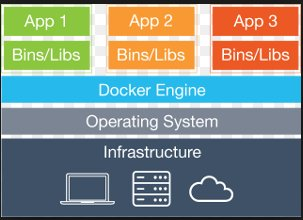
\includegraphics[scale=0.5]{docker.jpg}
\centering
\label{fig:instantaneo}
\end{figure}

A solução proposta por este trabalho, para resolver o problema de associação da evidência a sua origem de modo que o processo seja reprodutível, pausa a execução
do container e coleta um instantâneo da memória dos processos sob sua execução. Este processo é executado em intervalos de tempo conhecidos de modo a se ter uma
evolução da história da memória dos processos. Em um sistema derivado do linux (Ubuntu 14.04) isso foi atingido via cópia do diretório ``\\proc'' relacionado 
aos processos sob o ``cgroup'' associado ao container e salvo em disco. Para relacionar o instantâneo a sua origem, usamos como nome do arquivo contendo o instantâneo 
da memória a combinação do hash da imagem e o hash do container como mostrado na Figura 2.

\begin{figure}[h!]
\caption{Evidência salva - hash do container e imagem}
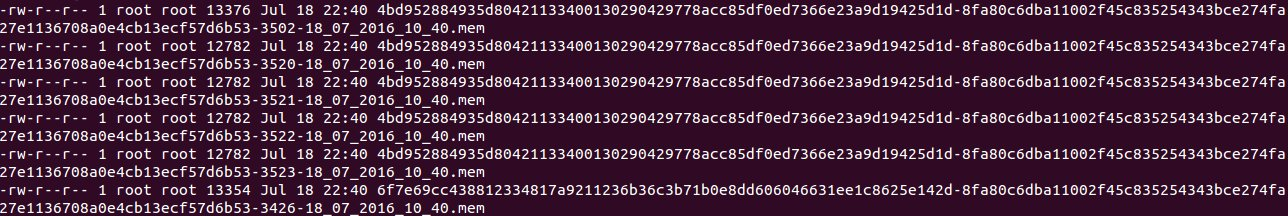
\includegraphics[scale=0.3]{snapshot.jpg}
\centering
\label{fig:instantaneo}
\end{figure}

As técnicas forenses praticadas hoje estão voltadas para a obtenção da informação em sua totalidade, seja via cópia bit a bit, seja por remoção do hardware \cite{Simou2014}
\cite{Bem2008}. Tais práticas tem levado ao crescente volume de dados que os investigadores tem que analisar. Há uma vertente na comunidade chamada ``sniper 
forensics'' onde se coleta e armazena o suficiente para a investigação. A solução proposta por este trabalho acompanha esta tendência, a questão foi definir a quantidade 
de dados ``suficiente'' para uma investigação. Decidimos que ``suficiente'' seria a quantidade necessária para descrever o sistema antes e depois do ataque. A idéia é 
implementar um log rotativo de instantâneos de memória cobrindo uma quantidade de tempo configurável, integrar a solução com algum sistema de detecção de ameaça de modo
que, ao detectar um ataque, o log passa de rotativo a completo assim permitindo que se conheça o sistema antes e depois do ataque como mostrado na Figura 3. 

\begin{figure}[h!]
\caption{Janela deslizante de coleta de evidência}
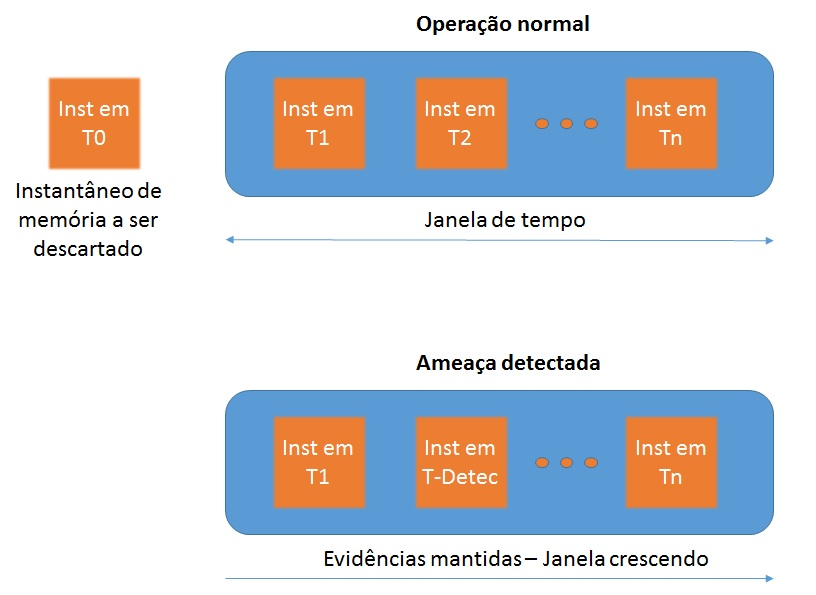
\includegraphics[scale=0.5]{janela.jpg}
\centering
\label{fig:janela}
\end{figure}

De modo a não violar a jurisdição de outros países ou a privacidade de outros usuários por causa do caráter multi-inquilino e multi-jurisdição das arquiteturas em núvem pública,
a solução proposta por este trabalho foi o de armazenar a evidência em um local físico fora da nuvem utilizando como transporte conexão segura. Outro ponto importante é 
garantir a cadeia de custódia da evidência ou seja, garantir que a evidência não foi destruída, alterada ou acessada por qualquer pessoa. Assim a solução proposta por este 
trabalho usará de armazenamento físico fora da nuvem, o transporte será feito por TLS e o acesso a evidência será controlado.

Tendo a implementação sido bem sucedida conseguiremos analisar e identificar as formas de ataque enumeradas nos objetivos.\\

\textbf{Limitações da solução}

Ameaças das quais estamos focando neste trabalho usam técnicas que permitem passar desapercebidas pelo processo de detecção de ameaças. Algumas delas são, 
adulteração da lista de processos ativos em uma máquina, se fazer passar por um processo válido ou se fazer passar por uma biblioteca válida \cite{Case2014}. Por isso, 
mesmo que haja uma integração com alguma forma de detecção de ameaça para a mudança do armazenamento de janela para o armazenamento total, acreditamos que ainda é 
necessária a capacidade de acionamento manual.

A solução esta focada em coletar informações de memória do espaço de memória do usuário assim, mesmo que ela ajude na investigação de ameaças que realizem manipulação direta
dos objetos do Kernel ( \textit{D.K.O.M. - Direct Kernel Object Manipulation} ) Kernel space no host não se beneficia da associação com o container.\\

\textbf{Esquema da solução}

A solução completa com todos os elementos descritos anteriormente pode ser visto na figura 4

\begin{figure}[h]
\caption{Solução completa}
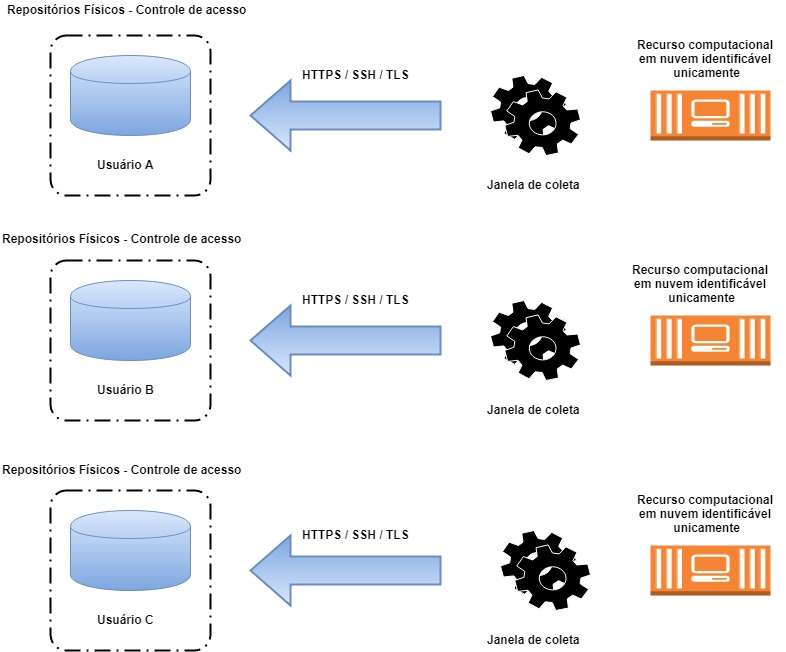
\includegraphics[scale=0.5]{solucao.jpg}
\centering
\label{fig:Solucao}
\end{figure}

% ----------------------------------------------------------
% Análise dos resultados
% ----------------------------------------------------------
\chapter{Análise dos Resultados}

Aqui a análise dos resultados \cite{Quick2014}

% ---
% Finaliza a parte no bookmark do PDF
% para que se inicie o bookmark na raiz
% e adiciona espaço de parte no Sumário
% ---
\phantompart

% ----------------------------------------------------------
% ELEMENTOS PÓS-TEXTUAIS
% ----------------------------------------------------------
\postextual

% ----------------------------------------------------------
% Referências bibliográficas
% ----------------------------------------------------------
\bibliography{abntex2-modelo-references}

%---------------------------------------------------------------------
% INDICE REMISSIVO
%---------------------------------------------------------------------

\phantompart

\printindex


\end{document}
